\documentclass[12zpt]{article}
\usepackage[spanish, es-tabla]{babel}
\usepackage[top=2cm, bottom=2cm,left=2cm, right=2cm]{geometry}
\usepackage[utf8x]{inputenc}
\usepackage{amsmath}
\usepackage{enumerate}
\usepackage{graphicx}
\graphicspath{ {images/} }
\usepackage{xcolor}
\usepackage{hyperref}
\hypersetup{
colorlinks=false,
linkbordercolor={white}
}

\usepackage{parskip}
\usepackage{listings}
\usepackage{courier}
\lstset{
	numbers=left, % Muestra el número de linea
	stepnumber=1, % Empieza por el 1
	basicstyle=\footnotesize\ttfamily, % Standardschrift
	%numbers=left,               % Ort der Zeilennummern
	numberstyle=\tiny,          % Stil der Zeilennummern
	%stepnumber=2,               % Abstand zwischen den Zeilennummern
	numbersep=5pt,              % Abstand der Nummern zum Text
	tabsize=2,                  % Groesse von Tabs
	extendedchars=true,         %
	breaklines=true,            % Zeilen werden Umgebrochen
	keywordstyle=\color{red},
		frame=b,         
	%        keywordstyle=[1]\textbf,    % Stil der Keywords
	%        keywordstyle=[2]\textbf,    %
	%        keywordstyle=[3]\textbf,    %
	%        keywordstyle=[4]\textbf,   \sqrt{\sqrt{}} %
	stringstyle=\color{white}\ttfamily, % Farbe der String
	showspaces=false,           % Leerzeichen anzeigen ?
	showtabs=false,             % Tabs anzeigen ?
	xleftmargin=17pt,
	framexleftmargin=17pt,
	framexrightmargin=5pt,
	framexbottommargin=4pt,
	%backgroundcolor=\color{lightgray},
	showstringspaces=false      % Leerzeichen in Strings anzeigen ?        
}
\lstloadlanguages{% Check Dokumentation for further languages ...
	   %[Visual]Basic
	   %Pascal
	   %C
	   %C++
	   %XML
	   %HTML
	   Java
}
  %\DeclareCaptionFont{blue}{\color{blue}} 

%\captionsetup[lstlisting]{singlelinecheck=false, labelfont={blue}, textfont={blue}}
\usepackage{caption}
\DeclareCaptionFont{white}{\color{white}}
\DeclareCaptionFormat{listing}{\colorbox[cmyk]{0.74, 0.22, 0.0,0.21}{\parbox{\textwidth}{\hspace{15pt}#1#2#3}}}
\captionsetup[lstlisting]{format=listing,labelfont=white,textfont=white, singlelinecheck=false, margin=0pt, font={bf,footnotesize}}

\newcommand{\img}[1]{
\noindent\makebox[\textwidth][c]{\includegraphics[width=1\textwidth,]{#1}}%
}
\usepackage{fancyhdr} 
\pagestyle{fancy}
\fancyhf{}
\fancyhead[L]{\footnotesize Universidad de Granada} %encabezado izquierda
\fancyhead[R]{\footnotesize ETSIIT}   % dereecha
\fancyfoot[R]{\footnotesize Sistemas Gráficos}  % Pie derecha
\fancyfoot[C]{\thepage}  % centro
\fancyfoot[L]{\footnotesize 2018/2019}  %izquierda
\renewcommand{\footrulewidth}{0.4pt}

\begin{document}

%%%%%%%%%%%%%%%%%%%%%%%%%%%%%%%%%% PORTADA %%%%%%%%%%%%%%%%%%%%%%%%%%%%%%%%%%%%%%%%%%%%
																					%%%
\begin{center}																		%%%
\newcommand{\HRule}{\rule{\linewidth}{0.5mm}}									%%%\left
 																					%%%
\begin{minipage}{0.48\textwidth} \begin{flushleft}

\includegraphics[scale = 0.42]{logo1.png}
\end{flushleft}\end{minipage}
\begin{minipage}{0.48\textwidth} \begin{flushright}

\includegraphics[scale = 0.35]{logo2.png}
\end{flushright}\end{minipage}

													 								%%%
\vspace*{-1.5cm}								%%%
																					%%%	
\textsc{\huge Universidad de Granada\\ \vspace{5px} ETSIIT}\\[1.5cm]	

\textsc{\LARGE Sistemas Gráficos}\\[1.5cm]													%%%

%%%
    																				%%%
 			\vspace*{1cm}																		%%%
																					%%%
\HRule \\[0.4cm]																	%%%
{ \huge \bfseries Manual de usuario - Práctica 2}\\[0.4cm]	%%%
 																					%%%
\HRule \\[1.5cm]																	%%%
 																				%%%
																					%%%
\begin{minipage}{0.46\textwidth}													%%%
\begin{center} \large															%%%	
\textbf{Autores:} Guillermo Bueno Vargas\\
Juan Carlos Ruiz García,\\
\textbf{Emails:} guillergood@correo.ugr.es, jcarlosruiz95@correo.ugr.es,\\
\textbf{Githubs:} Guillergood, juanka1995\\ 
\end{center}																		%%%
\end{minipage}		
																	%%%
\vspace{7cm} 																				
\begin{center}																					
{\large \today}																	%%%
 			\end{center}												  						
\end{center}							 											
																					
\newpage																		
%%%%%%%%%%%%%%%%%%%% TERMINA PORTADA %%%%%%%%%%%%%%%%%%%%%%%%%%%%%%%%

%%%%%%%%%%%%%%%%%%%% INDICE %%%%%%%%%%%%%%%%%%%%%%%%%%%%%%%%

\tableofcontents

\newpage

\section{Instalación}
Este proyecto no requiere de una instalación como tal, tan solo será necesario lanzar un \textbf{servidor HTTP} sobre la carpeta principal del proyecto.
Necesitaremos tener instalado \textbf{Python} y podremos iniciar nuestro servidor de \textbf{dos formas} dependiendo de la versión de Python que utilicemos:

\begin{enumerate}
	\item \textbf{Python 2:} \textit{python ­-m SimpleHTTPServer} 
	\item \textbf{Python 3:} \textit{python ­-m http.server} 
\end{enumerate}

\noindent\makebox[\textwidth][c]{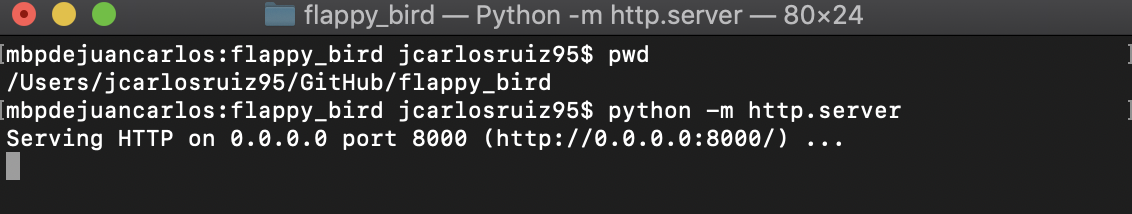
\includegraphics[width=0.8\textwidth,]{1.png}}

Una vez hecho esto bastaría con abrir nuestro navegador y acceder a la dirección \textit{http://localhost:8000}. Una vez aqui accedemos a la 
carpeta \textit{flappy\_bird} y automáticamente se lanzaría el juego.

\noindent\makebox[\textwidth][c]{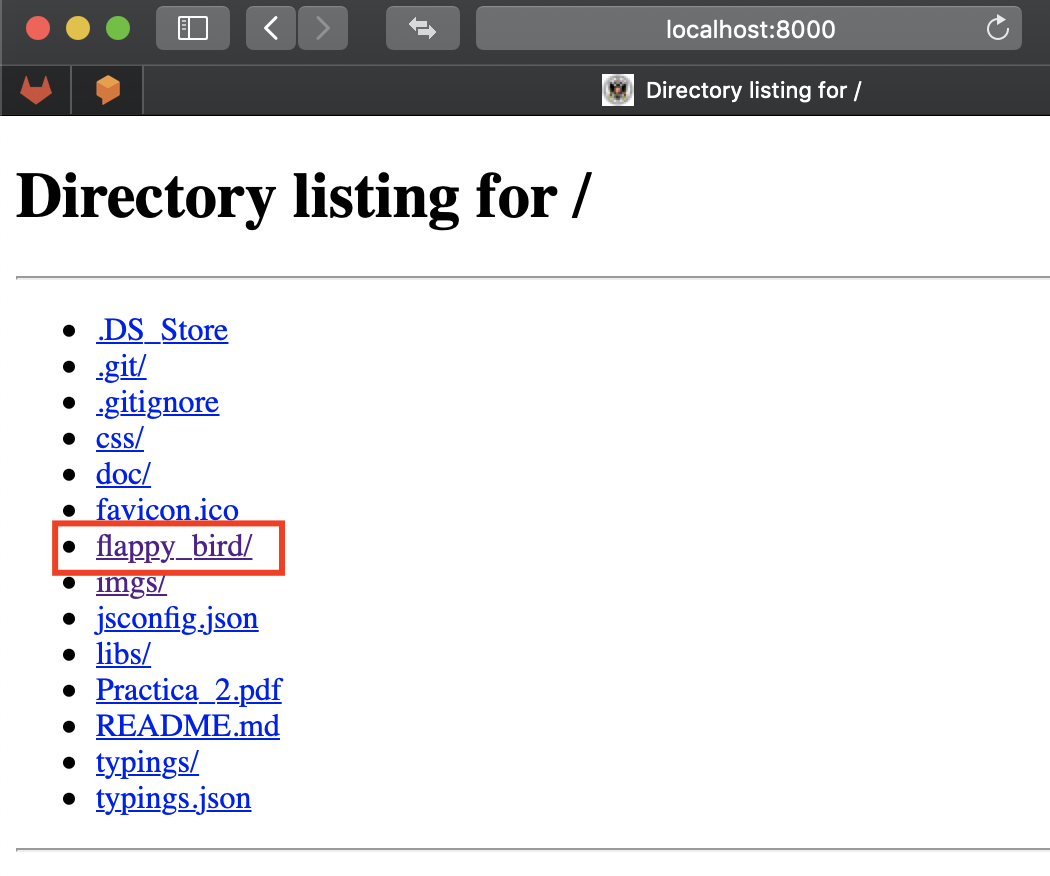
\includegraphics[width=0.5\textwidth,]{2.png}}
\noindent\makebox[\textwidth][c]{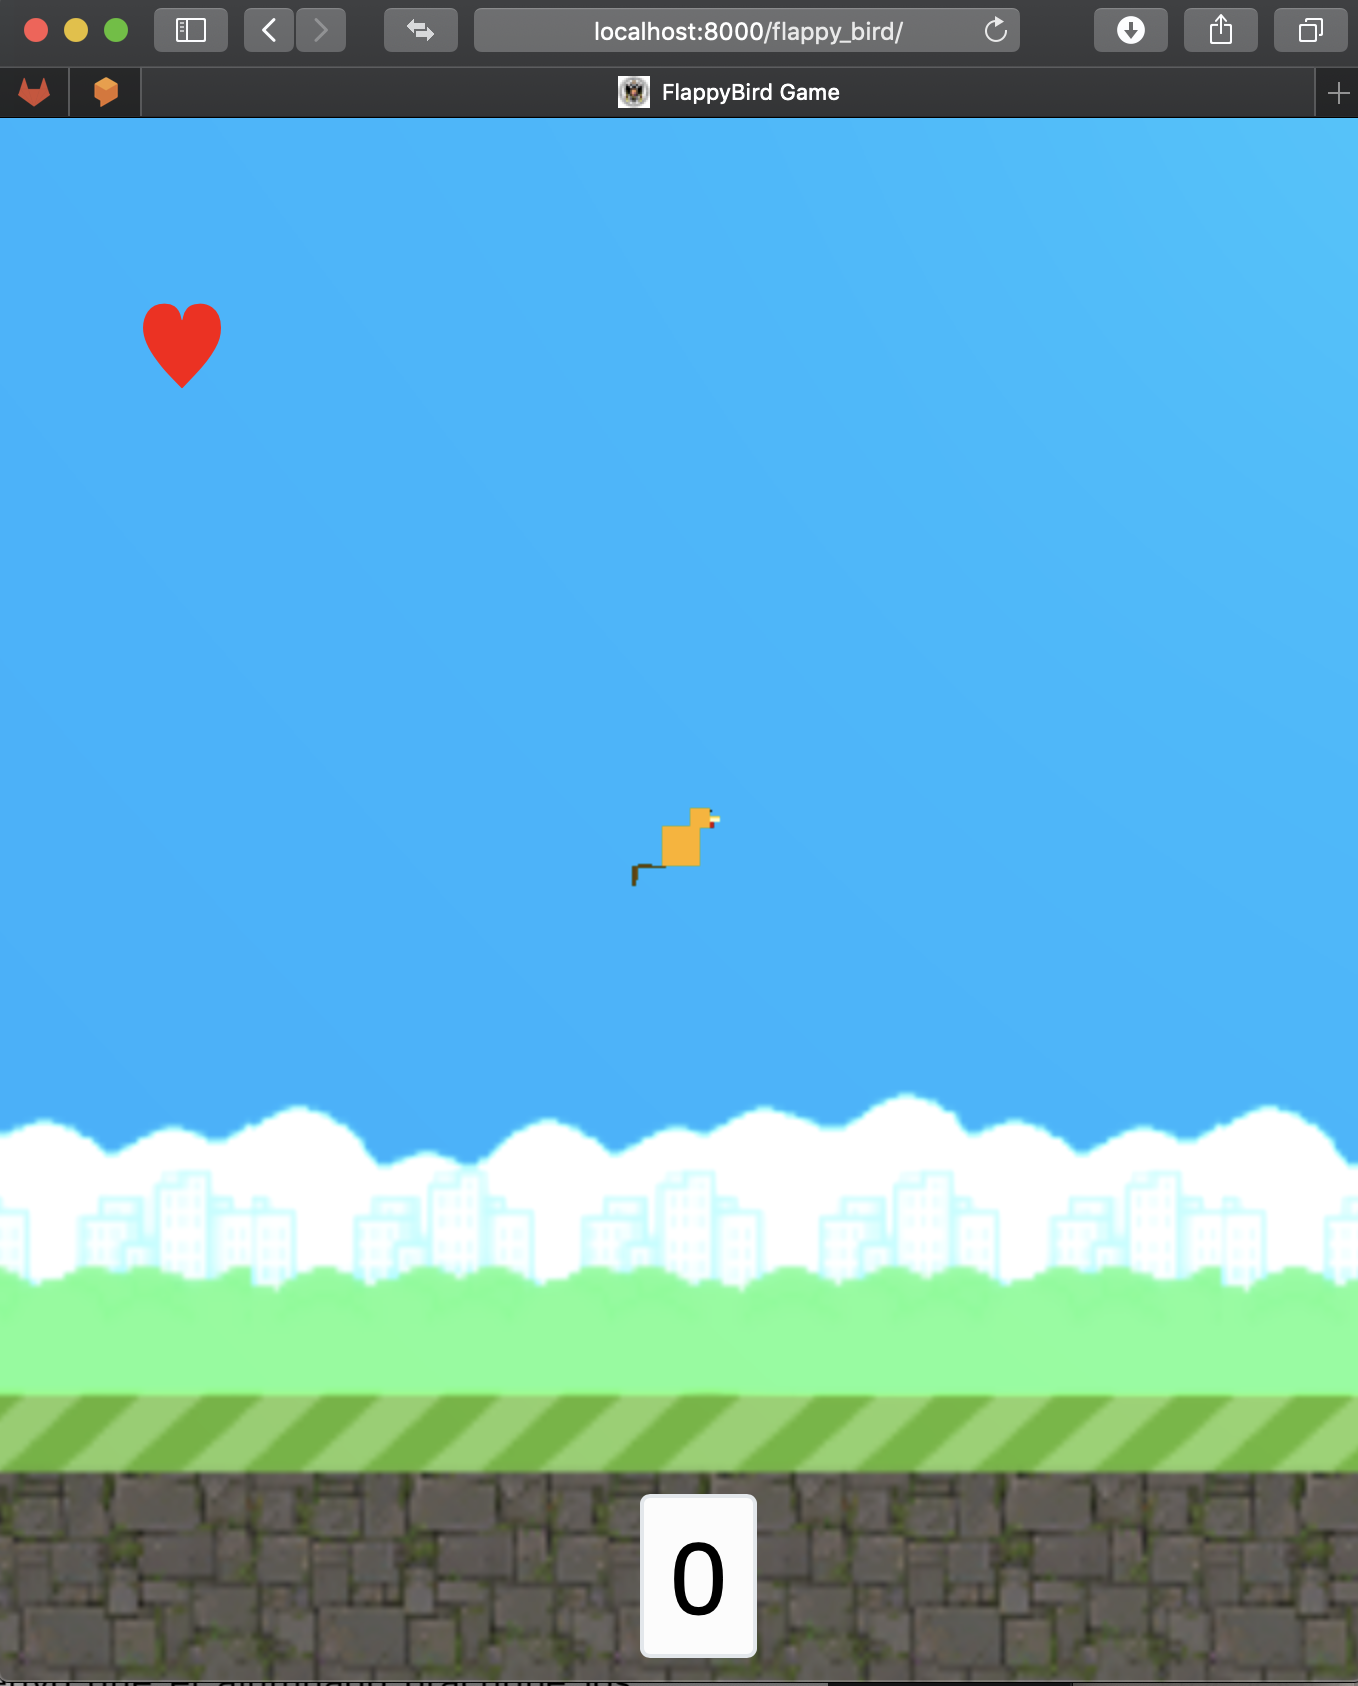
\includegraphics[width=0.4\textwidth,]{3.png}}


\section{Controles}
Para controlar a nuestro personaje, podrémos utilizar \textbf{2 alternativas:}

\begin{enumerate}
	\item \textit{Botón izquierdo del ratón}.
	\item \textit{Barra espaciadora del teclado}.
\end{enumerate}

El funcionamiento es muy simple, ya que el jugador deberá pulsar repetidamente una de estas dos opciones para conseguir la mayor puntuación posible.


\section{Tipos de bonus}
Durante la ejecución del juego existirán \textbf{2 tipos} de bonus:

\begin{enumerate}
	\item \textbf{Corazón:} el corazón dará a nuestro personaje en el juego una vida extra, permitiendonos cometer algún que otro fallo.
\end{enumerate}
\noindent\makebox[\textwidth][c]{
\includegraphics[width=0.1\textwidth,]{4.png}} 

\begin{enumerate}
	\item \textbf{Moneda:} La moneda \textbf{incrementará x2} la puntuación obtenida por cada obstaculo superado, pero a su vez hará que el personaje
	tenga un tamaño un \textbf{1\% mayor}, por lo que será más dificil superar los obstáculos.
\end{enumerate}
\noindent\makebox[\textwidth][c]{
\includegraphics[width=0.1\textwidth,]{5.png}}


\section{Marcadores}

Existirán \textbf{2 tipos} de marcadores:

\begin{enumerate}
	\item \textit{Durante la partida:} este marcador aparecerá en la parte inferior de la pantalla y será el que nos indicará la puntuación que llevamos hasta le momento.
\end{enumerate}
\noindent\makebox[\textwidth][c]{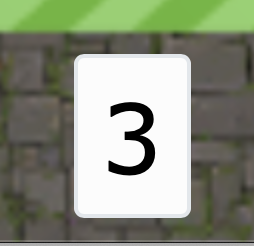
\includegraphics[width=0.15\textwidth,]{7.png}}

\begin{enumerate}
	\item \textit{Al finalizar la partida:} este marcador aparecerá cuando el jugador pierda todas sus vidas y mostrará un resumen de la puntuación obtenida en la partida 
	previamente jugada. Además nuestro navegador guardará la mejor puntuación que hayamos obtenido en todas las partidas que hayamos jugado, pudiendo constrastar así la puntación 
	obtenida con la mejor hasta el momento.
\end{enumerate}
\noindent\makebox[\textwidth][c]{
\includegraphics[width=0.6\textwidth,]{6.png}}

%%%%%%%%%%%%%%%%%%%% TERMINA INDICE %%%%%%%%%%%%%%%%%%%%%%%%%%%%%%%%

\end{document}
